\documentclass[12pt,spanish,oneside,letterpaper]{book}
%\usepackage{uarial}
%\renewcommand{\familydefault}{\sfdefault}
% Configuración de idioma y codificación de caracteres
\usepackage[spanish, es-tabla]{babel}
\usepackage[utf8x]{inputenc}
\usepackage[T1]{fontenc}
\usepackage{colortbl}
\usepackage{tcolorbox}
% Números de línea para facilitar la revisión
%\usepackage{lineno}
%\linenumbers

\usepackage[table]{xcolor} % Paquete para color en tablas
\usepackage{colortbl} % Para colorear celdas individuales

\definecolor{lightgray}{gray}{0.9} % Gris claro
\definecolor{mediumgray}{gray}{0.8} % Gris medio
\definecolor{softblue}{RGB}{220, 230, 241} % Azul suave

\usepackage{fancyhdr}
\usepackage{xcolor}
\usepackage{pdfpages}
\usepackage{graphicx}
% \usepackage{amsmath}
\usepackage{booktabs}
\usepackage{caption}
\usepackage[algo2e,algoruled,lined,linesnumbered,spanish]{algorithm2e}
\usepackage{hyperref}
\usepackage{amsmath,amssymb,amsfonts,latexsym,cancel}
\usepackage{float}

\graphicspath{Imagenes/}
% Punto en lugar de coma para separar decimales
\spanishdecimal{.}
% Configuración del pie de Figuras y Tablas
\captionsetup{font=footnotesize,labelfont=bf,labelsep=period}
%\captionsetup[table]{position=top}

% Encabezado
\pagestyle{fancy}
\fancyhead[L]{}
\fancyhead[R]{\nouppercase\leftmark}

\usepackage{subfigure,graphicx}

% Nombres de Índices
\renewcommand{\contentsname}{Tabla de contenido}
\renewcommand{\listfigurename}{Índice de ilustraciones}
\renewcommand{\listtablename}{Índice de tablas}
\usepackage[letterpaper, margin=1.25in]{geometry}

\begin{document}
% Portada en un archivo externo en formato PDF
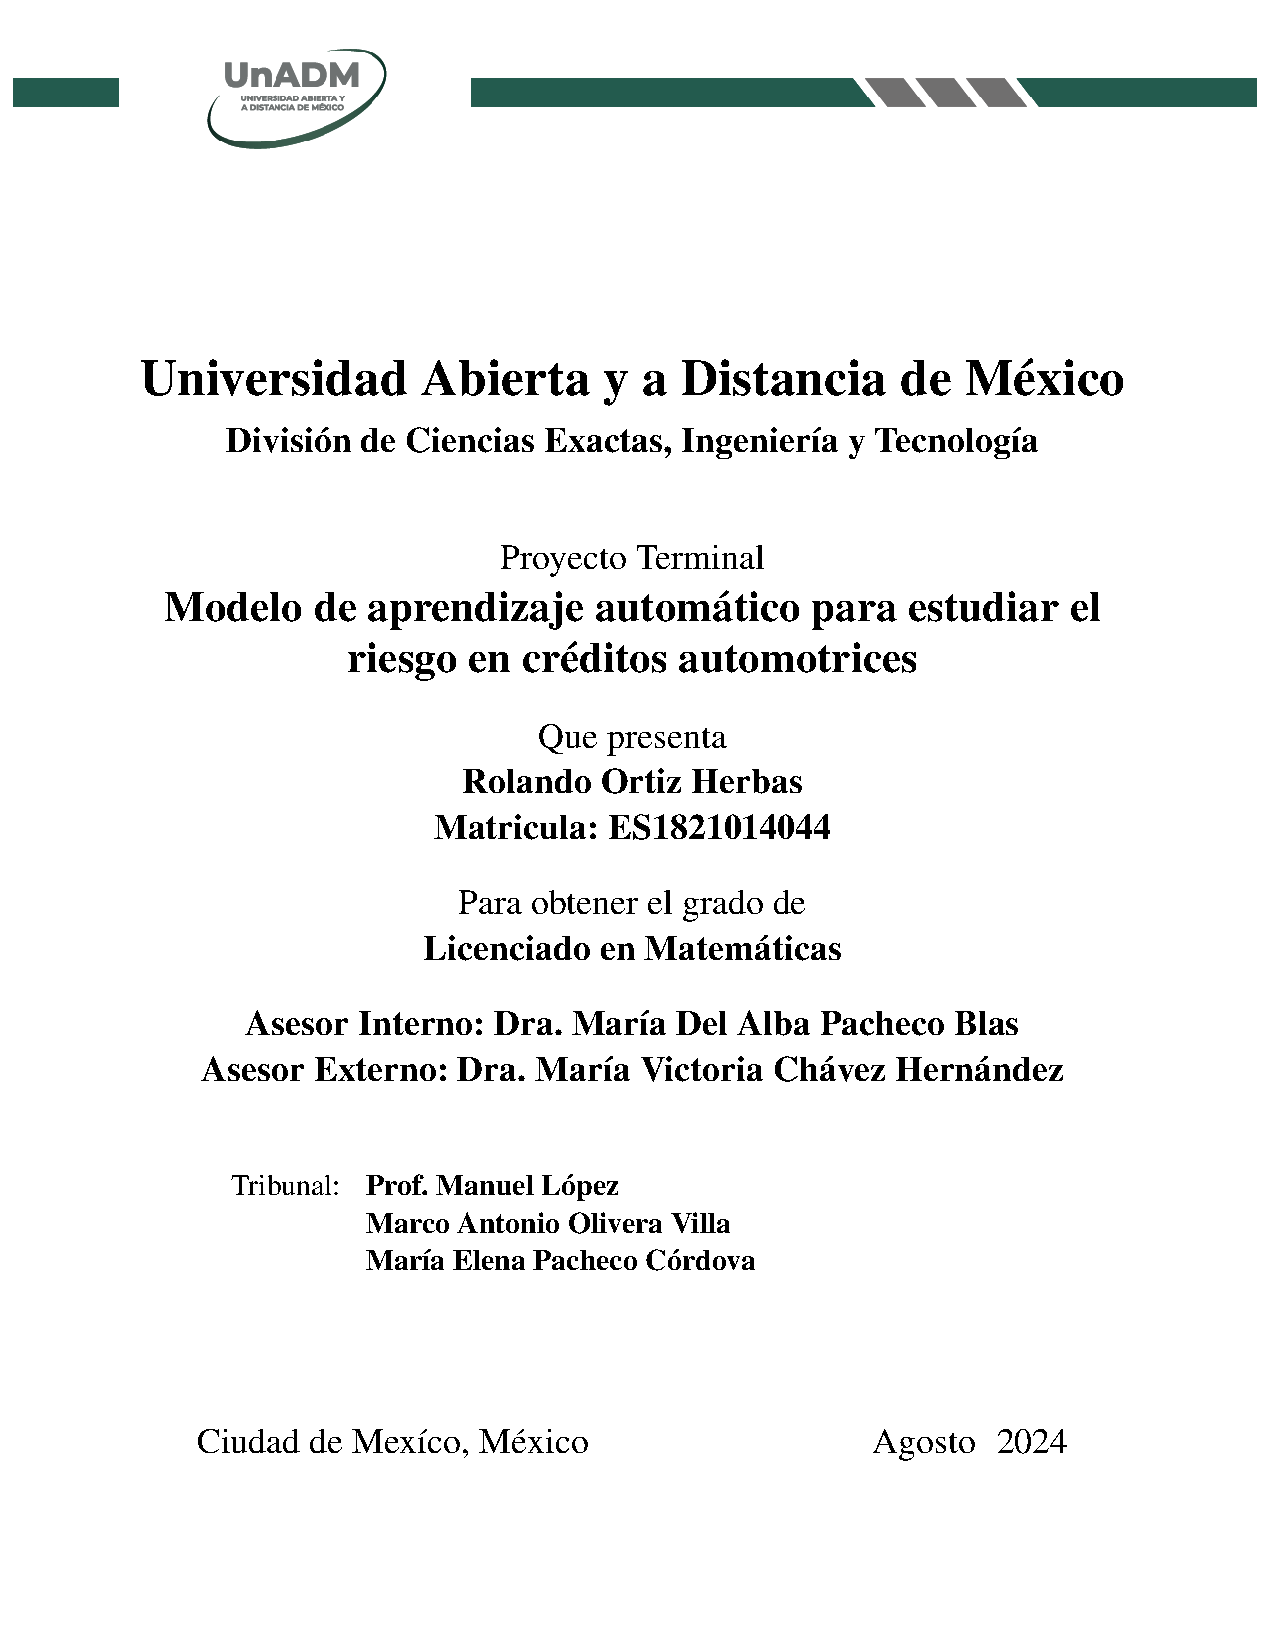
\includepdf[pages=-]{Portada}

% Hoja en blanco
% \leavevmode\thispagestyle{empty}\newpage

\setcounter{page}{1}
\pagenumbering{roman}
\addcontentsline{toc}{chapter}{Tabla de contenido}
\tableofcontents
\newpage
\addcontentsline{toc}{chapter}{Índice de Figuras}
\listoffigures
\newpage
\addcontentsline{toc}{chapter}{Índice de Tablas}
\listoftables
\newpage
%\setcounter{page}{1}
%\pagenumbering{arabic}

%*****************************************************************************%
%***************************** C A P Í T U L O S *****************************%
%*****************************************************************************%
% Obligatorio
\addcontentsline{toc}{chapter}{{}Dedicatoria}

\chapter*{Dedicatoria}

\vspace*{-8mm}

{\color{blue}
Mi Dedicatoria
}
% Obligatorio
\addcontentsline{toc}{chapter}{{}Agradecimientos}

\chapter*{Agradecimientos}

\vspace*{-8mm}

Mi agradecimiento.\medskip



%\setcounter{page}{1}
%\pagenumbering{arabic}
% Obligatorio
\addcontentsline{toc}{chapter}{{}Resumen}

\chapter*{Resumen}

\vspace*{-8mm}

El uso de la inteligencia artificial, y en particular del aprendizaje automático (Machine Learning), ha transformado la evaluación de riesgos en préstamos, al considerar múltiples factores como historiales de crédito y tendencias del mercado. Estos modelos permiten predecir con 
mayor precisión la probabilidad de incumplimiento, lo que ayuda
 a las instituciones financieras a ajustar las tasas de interés y asignar recursos de manera eficiente. Además, su capacidad de adaptación a cambios en los datos y condiciones del mercado los hace flexibles. No obstante, es fundamental enfrentar retos éticos y 
de privacidad para asegurar un uso justo. \medskip

Palabras clave: inteligencia artificial, aprendizaje automático, evaluación de riesgos, préstamos, previsión de incumplimiento, adaptación, ética, privacidad.



\newpage
\setcounter{page}{1}
\pagenumbering{arabic}
% Obligatorio
\chapter{Introducción}\label{cap1:Introducción}

\section{Antecedentes}



El presente proyecto tiene como objeto el elaborar un modelo que nos permita determinar un 
conjunto de variables que nos permitan clasificar a un cliente como confiable para ser un 
sujeto de crédito o no. Este proceso también se llevará a cabo durante el tiempo que este 
pagando el crédito que se le otorgó por lo que es estatus del cliente puede variar en el 
tiempo. \medskip

Este estudio se esta realizando para la empresa  “Wireless And Mobile Telecommunications, S. de R.L. de C.V.” 
que  es una consultora en el área de telecomunicaciones e inteligencia artificial. \medskip

“Wireless And Mobile Telecommunications”, busca potenciar su capacidad de gestión de riesgos 
en el ámbito crediticio. Con una base de clientes en constante expansión, la empresa se 
encuentra en la encrucijada de equilibrar el acceso al crédito para sus clientes con la 
necesidad de salvaguardar su salud financiera. \medskip

El contexto actual destaca la importancia de adoptar enfoques innovadores, y es en este marco 
que surge la iniciativa de implementar un modelo de riesgo de créditos basado en 
machine learning. Este enfoque moderno permitirá evaluar de manera más precisa y 
eficiente la capacidad crediticia de sus clientes, optimizando así el proceso de toma de 
decisiones. \medskip

El modelo se centrará en el análisis de datos, utilizando algoritmos de machine learning para 
identificar patrones relevantes que influyen en la solvencia crediticia. La integración de datos 
internos mejorará la robustez del modelo, ofreciendo a la empresa una herramienta ágil y 
precisa para evaluar el riesgo asociado a cada solicitud de crédito. \medskip

La implementación de este modelo no solo fortalecerá la posición financiera de la empresa, 
sino que también mejorará la experiencia del cliente al agilizar el proceso de aprobación de 
créditos. La capacidad de ofrecer respuestas rápidas y personalizadas a las solicitudes de 
crédito no solo aumentará la satisfacción del cliente, sino que también respaldará el 
crecimiento continuo de la empresa en un entorno competitivo.
\section{Justificación}

Un estudio realizado por “Wireless And Mobile Telecommunications, S. de R.L. de C.V.” 
reveló que, de una muestra de 1000 clientes, 142 incumplieron con 
el pago de sus créditos automotrices. \medskip

Dado que cada crédito promedio asciende a 300,000 pesos M.N. y, 
asumiendo que los clientes morosos dejaron de pagar el 50% 
del crédito, la pérdida estimada para la empresa
asciende a 21,000,000 pesos M.N. (142 clientes * 150,000 pesos M.N.). \medskip

Esta situación subraya la importancia de mejorar las
herramientas de evaluación de riesgo y control de morosidad.
Implementar soluciones avanzadas, como el uso de inteligencia artificial y modelos de aprendizaje automático, 
permitiría prever con mayor precisión los casos de incumplimiento 
y, por ende, reducir las pérdidas financieras. Además, una gestión proactiva del riesgo no solo optimiza la asignación de recursos, sino que también fortalece la estabilidad económica de la empresa en un entorno altamente competitivo.

\section{Objetivos}

\subsection{Objetivo general}

Desarrollar e implementar un modelo para la evaluación dinámica de la elegibilidad crediticia 
de los clientes , desde el inicio del crédito y a lo largo del tiempo, mediante periodos 
definidos de pago, con el fin de optimizar la toma de decisiones crediticias y fortalecer 
la salud financiera de la empresa.

\subsection{Objetivos específicos}

\begin{itemize}
\item Identificar variables clave para la evaluación inicial de la capacidad crediticia de los clientes al momento de solicitar un crédito.\medskip


\item Desarrollar un modelo que clasifique a los clientes como sujetos o no sujetos de crédito al inicio de la relación crediticia.\medskip

\item Establecer periodos definidos de análisis temporal, considerando variables como historial de pagos y comportamiento crediticio.\medskip

\item Recopilar y procesar datos relevantes de los clientes durante cada periodo definido, asegurando la actualización constante del modelo.\medskip

\item Refinar el modelo  a medida que se acumulan datos adicionales, mejorando la capacidad predictiva a lo largo del tiempo.\medskip

\item Evaluar la eficacia del modelo mediante métricas de desempeño, como precisión, sensibilidad y especificidad, para garantizar su confiabilidad en la toma de decisiones crediticias.\medskip

\item Implementar el modelo en el proceso de toma de decisiones crediticias, integrándolo de manera efectiva en las operaciones cotidianas.\medskip

\item Monitorear continuamente el rendimiento del modelo y realizar ajustes según sea necesario para adaptarse a cambios en el comportamiento crediticio de los clientes y en el entorno económico.\medskip

\end{itemize}
% Obligatorio.
\chapter{Marco investigativo}\label{cap2:Marco-Investigativo}

\section{Definición de conjunto de datos o dataset}

Una definición de aprendizaje automático es la siguiente : \medskip

“El machine learning traducido al español como aprendizaje automático es un subcampo de la 
Inteligencia Artificial que busca como construir programas de computadora que mejoran 
automáticamente adquiriendo experiencia” \cite{Arang} pág. 320 . \medskip

Usaremos indistintamente como sinónimo en lo futuro , “aprendizaje automático”   y  “machine learning”.

\begin{figure}[ht]
  \centering
  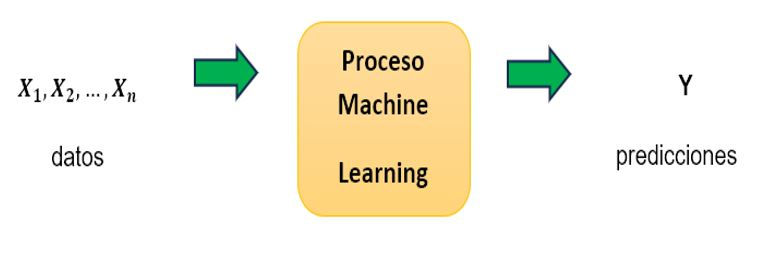
\includegraphics[width=10cm]{Imagenes/EsquemaML.JPG}
  \caption{Esquema Machine Learning}
  \label{fig:EsML}
\end{figure}

Un algoritmo de aprendizaje automático acepta como entrada un conjunto de datos también 
llamados dataset y después de un proceso realiza predicciones con estos datos \ref{fig:EsML} .\medskip



A la tabla completa de la Figura \ref{fig:Tblml}  la llamamos conjunto de datos (dataset), 
a las columnas en color amarillo le llamamos características y a la columna en color azul 
le llamamos variable objetivo y también se la conoce como etiqueta. \medskip

Como mencionamos anteriormente el aprendizaje supervisado cuenta con la columna de etiqueta y 
el aprendizaje no supervisado, no cuenta con esta columna.\medskip

Si la variable objetivo o característica son valores discretos , entonces le llamamos un 
problema de clasificación. Y si es un valor continuo le llamamos un problema de regresión.\medskip



De forma general los tipos de aprendizaje automático se pueden clasificar de la         
siguiente manera:\medskip

\begin{figure}[H]
    \centering
       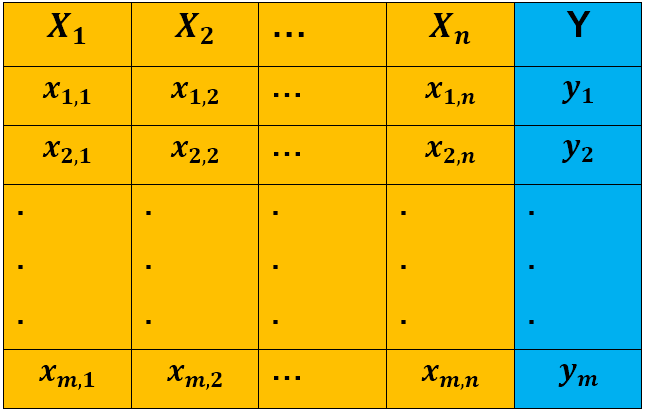
\includegraphics[width=12cm, height=7cm ]{Imagenes/TablaML.PNG}
      \caption{Conjunto de datos o dataset}
      \label{fig:Tblml}
  \end{figure} 


\subsection{Aprendizaje supervisado}
El modelo aprende con datos etiquetados, donde cada entrada tiene una respuesta conocida.\medskip

\subsection{Aprendizaje no supervisado}
El modelo trabaja con datos no etiquetados, descubriendo patrones y estructuras por sí mismo.\medskip


Estos tipos de aprendizaje ofrecen estrategias distintas para abordar desafíos en machine 
learning, cada uno con sus propias aplicaciones y utilidades específicas.\bigskip


\section{Clasificación}

La clasificación es un modelo supervisado en la cual el objetivo es predecir una 
etiqueta o clase para una entrada dada. En otras palabras, el modelo debe 
asignar una etiqueta categórica a las instancias basándose en características o 
atributos de los datos. \medskip

El modelo examina las características o atributos de los 
datos de entrada y crea una función o regla que relaciona esas características con la 
etiqueta de salida deseada. El objetivo final es que el modelo pueda generalizar esta 
relación aprendida para hacer predicciones precisas sobre nuevos datos no etiquetados. \medskip

En la Figura \ref{fig:Clasi} se muestra un ejemplo de un problema de clasificación de datos 
en dos o mas conjuntos que se relacionan con base en algunas características. La figura fue generada con 
ayuda del software Scikit-learn que puede graficar diferentes modelos de machine learning.


  \begin{figure}[H]
    \centering
       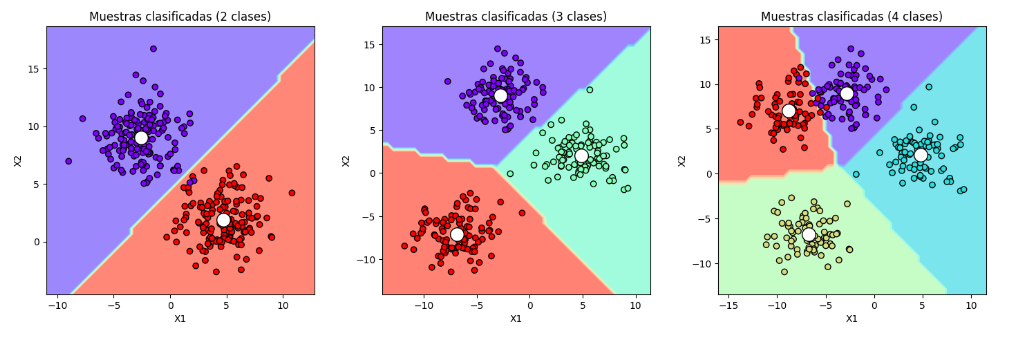
\includegraphics[width=12cm , height=5cm]{Imagenes/Clasificacion.PNG}
      \caption{Clasificación de un conjunto de datos}
      \label{fig:Clasi}
  \end{figure}
 

\section{Agrupamiento o Clustering}

El clustering o agrupamiento es un modelo no supervisado donde 
el objetivo es agrupar un conjunto de objetos en grupos, 
de manera que los objetos en el mismo grupo (o cluster) sean 
más similares entre sí que con los de otros grupos.\medskip

En la \ref{fig:Clast} se muestra un ejemplo de agrupamiento de datos 
usando el software Scikit-learn.


\begin{figure}[H]
    \centering
    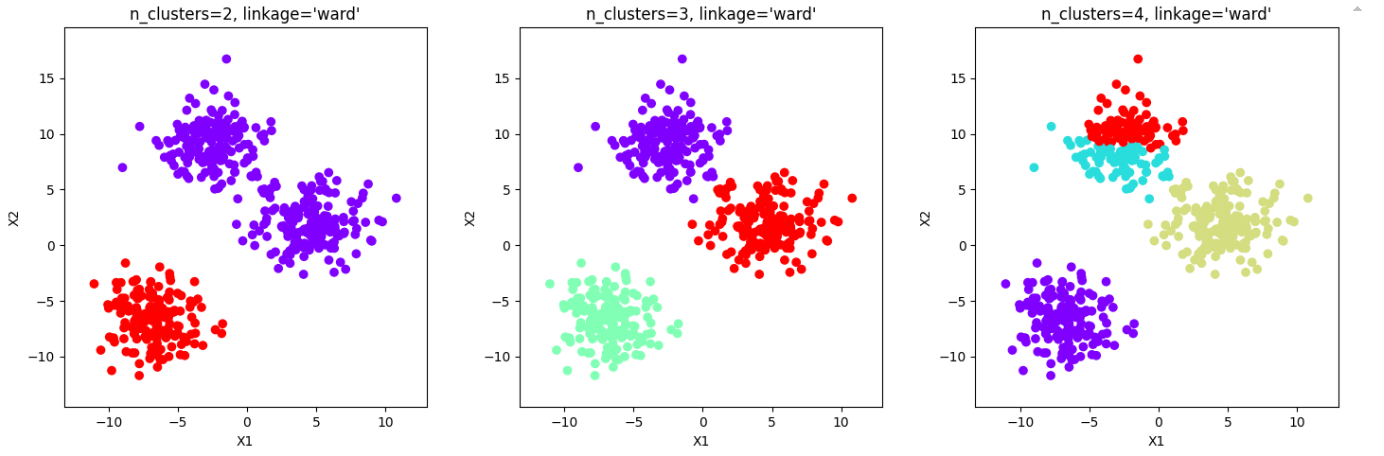
\includegraphics[width=12cm]{Imagenes/Clustering.PNG}
    \caption{Clustering o agrupamiento}
    \label{fig:Clast}
\end{figure}

\section{Regresión}
La regresión, es un modelo supervisado que busca entender la relación entre dos o más 
variables. En particular, se centra en proveer o regresar un valor numérico 
(la variable dependiente) en función de otras variables 
(llamadas variables independientes o predictores). \medskip

La regresión trata de encontrar la mejor línea o curva que represente la tendencia 
general de los datos. Esta línea o curva permite hacer predicciones sobre el valor de la 
variable dependiente cuando conoces los valores de las variables independientes. 
La figura \ref{fig:Reg1}  muestra varios tipos de regresión que modelan 
diferentes conjuntos de datos.\medskip



\begin{figure}[H]
    \centering
       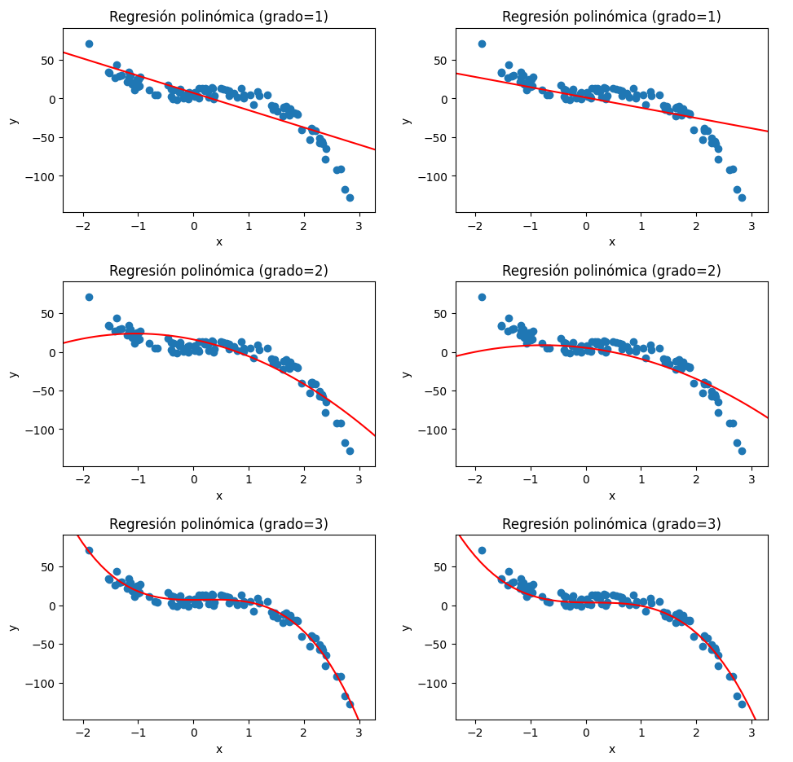
\includegraphics[width=10cm]{Imagenes/Regresion1.PNG}
      \caption{Regresión}
      \label{fig:Reg1}
\end{figure}



\section{Reducción de Dimensionalidad}

La reducción de dimensionalidad es una técnica fundamental en el análisis de datos que busca 
simplificar conjuntos de datos complejos manteniendo la mayor cantidad posible de información 
relevante. Una de las metodologías más populares para lograr esto es el 
Análisis de Componentes Principales (PCA, por sus siglas en inglés). \medskip

El Análisis de Componentes Principales (PCA) es una técnica estadística que se utiliza para 
reducir la cantidad de variables en un conjunto de datos mientras se conserva la mayor 
cantidad de variación en los datos originales. PCA transforma los datos originales en un 
nuevo sistema de coordenadas basado en componentes ortogonales, llamados componentes principales,
que son combinaciones lineales de las variables originales. \medskip

La reducción de  la dimensionalidad de los datos por lo tanto nos ayuda a 
simplificar el modelo matemático y, a su vez, disminuir los recursos computacionales, como 
el tiempo y el espacio de almacenamiento.\medskip




% Obigatorio. 
\chapter{Marco Teórico}\label{cap3:Marco-Teorico}

\section{Función logística}

La regresión logística es uno de los primeros algoritmos utilizados para resolver 
problemas de clasificación. Aunque su nombre pueda llevar a confusión al incluir la 
palabra ''Regresión'', este algoritmo no se emplea para problemas de regresión, sino 
para clasificación. Se aplica comúnmente en problemas de clasificación binaria 
\cite{Brownlee} Pág. 57. \medskip

La regresión logística es una técnica adecuada para clasificar si un cliente 
será un buen pagador debido a varias razones:

\begin{itemize}
    \item Es ideal para predecir dos posibles resultados, como ''buen pagador o mal pagador'' , ''confiable o no confiable''.
    \item Permite entender cómo diferentes características afectan la probabilidad de que un cliente sea "confiable o no confiable".
    \item No solo clasifica a los clientes, sino que también proporciona una probabilidad de que sean buenos pagadores, lo que facilita la toma de decisiones basadas en riesgo.
    \item Es un método rápido y eficiente para grandes volúmenes de datos.
\end{itemize}



La función logística \cite{Brownlee} Pág. 52, también conocida como la 
función sigmoide, es una función matemática comúnmente utilizada en
problemas de clasificación. Su forma característica es una curva en forma 
de ''S'' que transforma cualquier número real en un rango entre 0 y 1. \medskip


La función logística esta definida de la siguiente manera:

$$ \displaystyle y=logit(x)= \frac{1}{1+e^{-x}} $$


Y la grafica es: 

\begin{figure}[H]
    \centering
       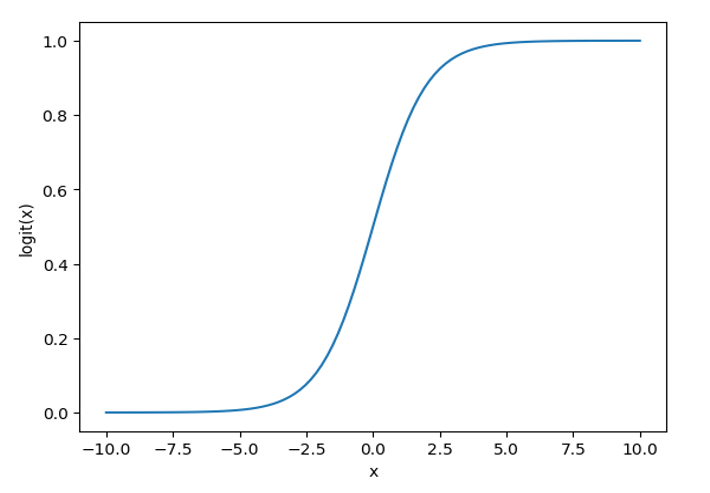
\includegraphics[width=12cm, height=7cm ]{Imagenes/Logit.PNG}
      \caption{Función logística , realizada en Scikit-Learn}
      \label{fig:logit}
  \end{figure} 

Esta claro que $ \displaystyle x \in ( \infty , {-}\infty ) \;  y \; logit(x) \in [0 , 1]$ \medskip
En general nuestra ecuación de trabajo será de la siguiente forma : \medskip

$$ \displaystyle y=B_0 + B_1X_1 + B_2X_2+ \dots + B_nX_n $$

 
Ahora tenemos muchos puntos de datos, por decir m puntos de datos en nuestro dataset. Para cada
punto de datos tendremos : \medskip

$$\displaystyle \sigma (y_i)= \frac{1}{1+e^{-y_i}} = \frac{1}{1+e^{-(B_0 + B_1X_{1i} + B_2X_{2i}+ \dots + B_nX_{ni})}} $$ \medskip

 Entonces,para cada punto, obtenemos un valor entre 0 y 1. Para hacer las preddicciones
 usamos el siguiente criterio: \medskip

\[
y = \left\{ \begin{array}{lcl}
1 & \mbox{ si } & \sigma (y) > 0.5 \\
& & \\
0 & \mbox{ si } & \sigma (y) \leq 0.5
\end{array}
\right.
\] \medskip

 Vamos a llamar $\sigma(y_i)$ como $p_i$ \\
 $$\displaystyle p_i =\widehat{y_i} = \sigma (y_i)= \frac{1}{1+e^{-y_i}} = \frac{1}{1+e^{-(B_0 + B_1X_{1i} + B_2X_{2i}+ \dots + B_nX_{ni})}} $$ \medskip
 
 \begin{itemize}
    \item $\displaystyle p_i = 1$ es la probabilidad de que la variable dependiente $\sigma (y_i)$ sea igual a 1 .
    \item $\displaystyle B_0 , B_1, B_2 , \dots,B_n$ son los parametros del modelo.
    \item $\displaystyle X_0 , X_{i1}, X_{i2} , \dots,X_{in}$ son las variables independientes del modelo.    
\end{itemize}

\section{Estimador de máxima verosimilitud}

Si tenemos n observaciones y para cada observación tenemos \medskip

$$ P(y_i =1 ) = \widehat{y_{i}}= \frac{1}{1+e^{-y_i}} = \frac{1}{1+e^{-(B_0 + B_1X_{1i} + B_2X_{2i}+ \dots + B_nX_{ni})}} $$  \medskip

Y la probabilidad de que $ y_i = 0 $ es:\medskip

$$ P(y_i =1 ) = \widehat{y_{i}}= \frac{1}{1+e^{-y_i}} = \frac{e^{(B_0 + B_1X_{1i} + B_2X_{2i}+ \dots + B_nX_{ni})}}{1+e^{(B_0 + B_1X_{1i} + B_2X_{2i}+ \dots + B_nX_{ni})}} $$  \medskip

La función de verosimilitud conjunta para todas las observaciones es: \medskip

$$ L(B_0 , B_1, B_2 , \dots,B_n) = \prod_{{i=1}}^{n} {\widehat{y_i}^{y_i}(1- \widehat{y_i})^{1- y_i}} $$ \medskip

Para simplificar la maximización, trabajamos con la log-verosimilitud , que es mas facil de manejar, Entonces \medskip

$$  \ell = ln(L(B_0 , B_1, B_2 , \dots,B_n)) =  ln(\prod_{i=1}^{n} \widehat{y_i}^{y_i}(1- \widehat{y_i})^{1- y_i}) = \sum_{i=1}^{n} (y_i ln(\widehat{y_i})+(1-y_i)ln(1- \widehat{y_i})) $$  \medskip

Para encontrar los estimadores de máxima verosimilitud, debemos maximizar la función 
log-verosimilitud con respecto a los parametros $(B_0 , B_1, B_2 , \dots,B_n)$ . Esto se logra calculando
las derivadas parciales de $ln$ con respecto a cada parámetro e igualando a cero:

$$ \frac{\delta \ell}{\delta B_j} =0 \, , \, para \, j\, =\, 0,1,\dots,n $$ \medskip

La derivada parcial con respecto a $B_0$ es \medskip

$$ \frac{\delta \ell}{\delta B_0} = \sum_{i=1}^{n} \displaystyle{\left(y_i - \frac{e^{(B_0 + B_1X_{1i} + B_2X_{2i}+ \dots + B_nX_{ni})}}{1+e^{(B_0 + B_1X_{1i} + B_2X_{2i}+ \dots + B_nX_{ni})}}\right)} $$ \medskip
Simplificando tenemos \\
$$ \frac{\delta \ell}{\delta B_0} = \sum_{i=1}^{n} (y_i - \widehat{y_i}) $$ \medskip

La derivada parcial con respecto a $B_j$ , para j = 1,2,\dots,n \medskip

$$ \frac{\delta \ell}{\delta B_j} = \sum_{i=1}^{n} \displaystyle{\left(y_i *X{ji} - \frac{ X{ji}* e^{(B_0 + B_1X_{1i} + B_2X_{2i}+ \dots + B_nX_{ni})}}{1+e^{(B_0 + B_1X_{1i} + B_2X_{2i}+ \dots + B_nX_{ni})}}\right)} $$ \medskip
Simplificando tenemos \\
$$ \frac{\delta \ell}{\delta B_j} = \sum_{i=1}^{n} (y_i - \widehat{y_i})* X_{ji} $$ \medskip

Estas derivadas muestran que cada parámetro se ajusta basándose en la diferencia entre los valores
observados $y_i$ y las probabilidades predichas $\widehat{y_i}$ , ponderadas por las variables correspondientes. \medskip
Para encontar los valores óptimos de $ B_0 , B_1, B_2 , \dots,B_n $ , estas ecuaciones se igualan a cero y se resuelven mediante
métodos numéricos. \medskip

Para resolver este sistema de ecuaciones usaremos el algoritmo de la gradiente descendente estocástico (SDG) , que es una variante del gradiente descendente clásico. El algoritmo es el siguiente:\\

\begin{itemize}
    \item Inicializacion:  inicializar $ B_0 , B_1, B_2 , \dots,B_n $  , por lo general en ceros.\medskip
    
    
    \item Actualizar los parámetros: basados en las reglas de actualización de la gradiente hacemos \\ \\
    $B_0 = B_0 + \alpha (y_i - \widehat{y_i}) \\
    Para \, B_j \, , \,  j = 1,2,\dots,n  \\
    B_j = B_j + \alpha * (y_i - \widehat{y_i}) * X_{ji}$.\medskip
    
    \item Repetir: se repite el proceso para cada observación en el conjunto de datos.\medskip

       
\end{itemize} \medskip

La convergencia y finalización del algoritmo se da cuando se cumple alguna de las siguientes condiciones
\begin{itemize}
\item El cambio en los parámetros $ B_0 , B_1, B_2 , \dots,B_n $  entre iteraciones 
es menor a una cantidad determinada
\item Se ha alcanzado un numero máximo de iteraciones
\end{itemize}





% Opcional. La contribución del estudiante podría ocupar más de un capítulo, en 
% cuyo caso los capítulos siguientes se reenumerarán.
\chapter{Metodología}\label{cap4:Metodologia}

\section{Metodología}

\begin{figure}[H]
    \centering
       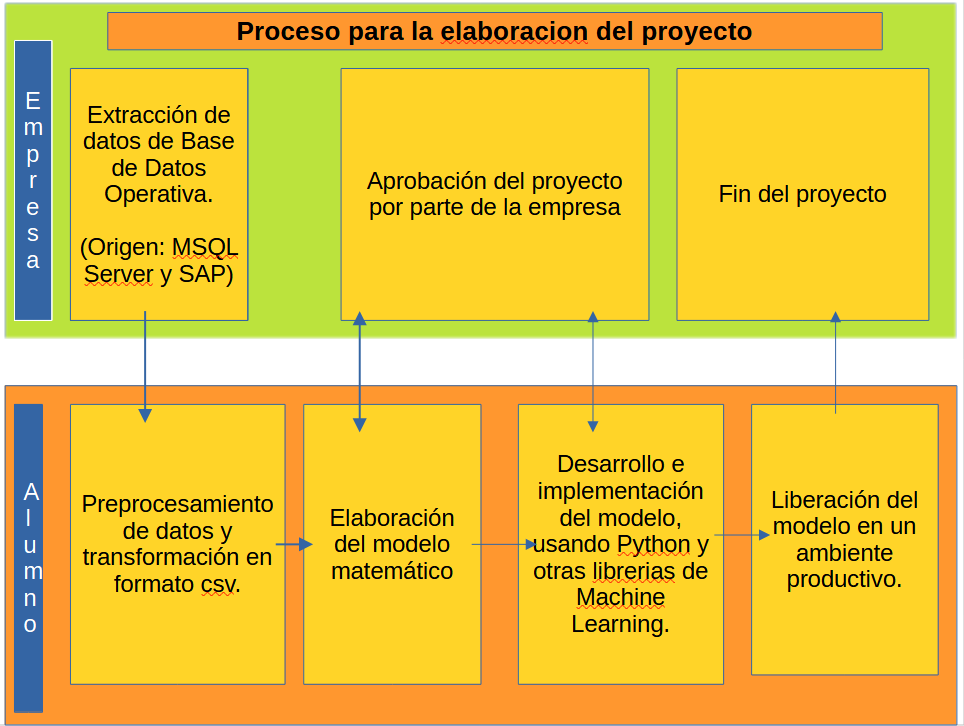
\includegraphics[width=12cm, height=7cm ]{Imagenes/Proceso_Proyecto.PNG }
      \caption{Metodología}
      \label{fig:meto}
\end{figure}

La metodología para realizar el proyecto se explica con la figura anterior.

\begin{itemize}
    \item La empresa proporciona la información con la que quiere que se desarrolle el modelo en formato Excel. \medskip
    \item Se recibe el archivo Excel y se realiza la limpieza y preprocesamiento de datos y se convierte a un formato de texto CSV , para usarlo como entrada por el algoritmo de aprendizaje . \medskip
    \item Se elabora el modelo y se interactúa con la empresa , hasta lograr un modelo este de acuerdo a sus necesidades. \medskip
    \item Una vez aprobado el modelo, se desarrolla el algoritmo usando el lenguaje de programación Python y otras librerías adicionales.\medskip
    \item El script o programa es evaluado por la empresa, la cual da su aprobación en cuanto a la funcionalidad requerida. \medskip
    \item Completado el anterior paso la empresa da su aprobación, con lo cual queda concluido el proyecto terminal. \medskip 
\end{itemize}

Una parte de dataset de trabajo es el siguiente :

\begin{figure}[H]
    \centering
       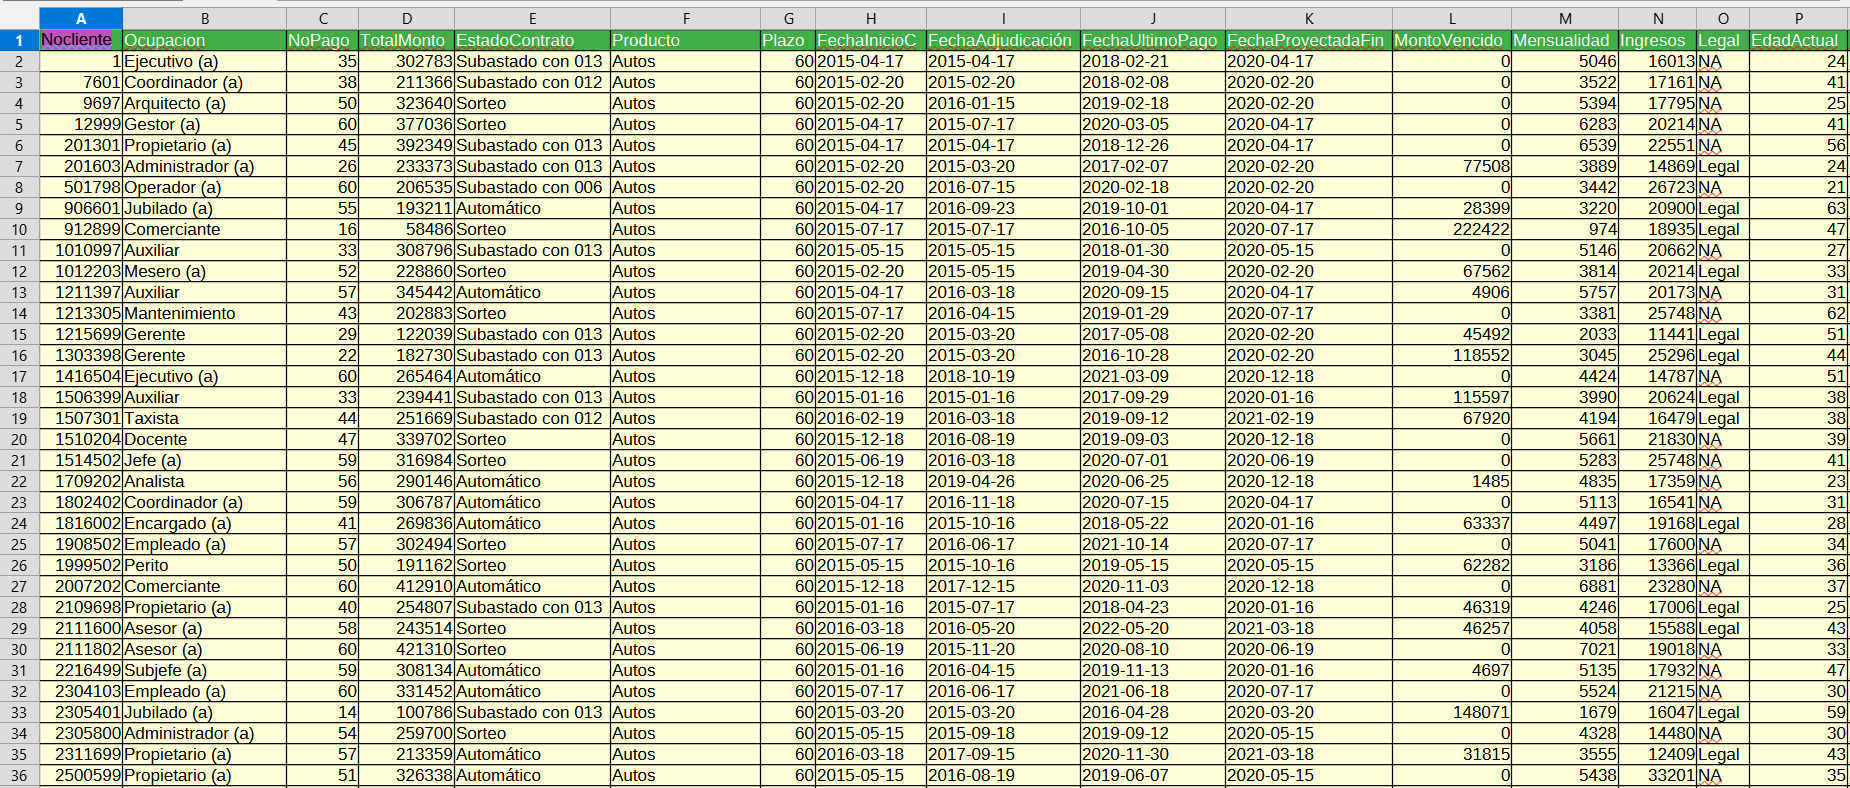
\includegraphics[width=12cm, height=10cm ]{Imagenes/Datos_Clientes1.PNG }
      \caption{Datos de los clientes (Bloque 1)}
      \label{fig:clis1}
\end{figure}
\newpage
\begin{figure}[H]
    \centering
       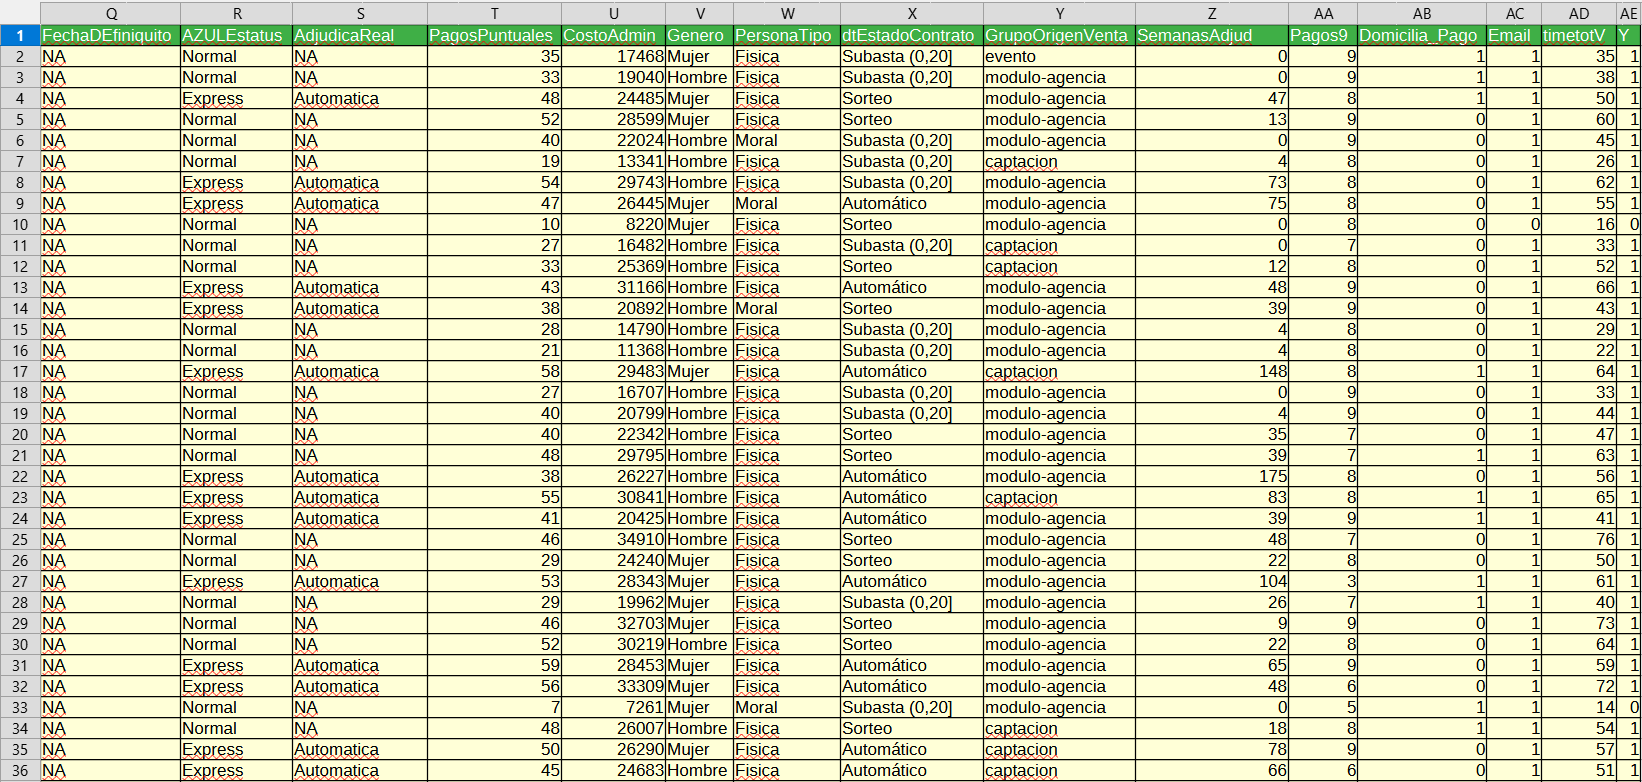
\includegraphics[width=12cm, height=10cm ]{Imagenes/Datos_Clientes2.PNG }
      \caption{Datos de los clientes (Bloque 2)}
      \label{fig:clis2}
\end{figure}
 
Descripción de las variables :

\begin{table}[H]
    \centering
    \begin{tabular}{|c|c|c|}
        \hline
        \rowcolor{softblue} % Fila color azul suave
        \textbf{Num} & \textbf{Nombre} & \textbf{Descripción} \\
        \hline
        % \rowcolor{lightgray} % Fila color gris claro
        \hline
        0 &	Nocliente &		Numero de cliente unico.   \\
        \hline
        1 &	Ocupacion &		Ocupación o profesión del cliente. 	\\
        \hline
        2 &  NoPago    &     Numero de pago actual. Entre 1 y 60 meses.  \\
        \hline
        3 &  TotalMonto  &    Cantidad  en moneda nacional, que se le prestó al cliente. \\
        \hline
        4 &  EstadoContrato &     Automático, Sorteo o Subasta.  \\
        \hline
        5 &   Producto  &         Auto, Inmueble, Moto (inicalmente solo se trabaja con Auto).  \\
        \hline
        6 &  Plazo     &          60 meses.  \\
        \hline
        7 &  FechaInicioC  &      Fecha de inicio de contrato.  \\
        \hline
        8 &  FechaAdjudicación &   Fecha de adjudicación del Auto.  \\
        \hline
        9 &   FechaUltimoPago &    Fecha de ultimo pago del prestamo. \\
        \hline
        10 &  FechaProyectadaFin &  Fecha proyectada de ultimo pago. \\
        \hline
        11 &  MontoVencido &        Monto vencido de pago.  \\
        \hline
        12 &  Mensualidad &         Cantidad a pagar mensualmente.  \\
        \hline
        % \rowcolor{mediumgray}
        13 &  Ingresos &    Ingreso mensual del cliente.  \\
        \hline
        % \rowcolor{mediumgray}
        14 &  Legal &     Si esta en estado normal o legal. \\
        \hline
        15 &  EdadActual &   Edad actual del cliente. \\
        \hline
        %\rowcolor{mediumgray}
        16 &  FechaDEfiniquito &    Fecha de finiquito. \\
        \hline
        17 &  AZULEstatus &   Express , normal. \\
        \hline
        %\rowcolor{mediumgray}
        18 &  AdjudicaReal &  Automática, normal , automática plus.\\
        \hline
        19 &  PagosPuntuales &      Numero de pagos puntuales en meses.  \\
        \hline
        20 &  CostoAdmin &    Costo administrativo por cliente. \\
        \hline
        21 &  Genero &       Mujer, Hombre u Otro . \\
        \hline
        22 &  PersonaTipo &   Si es persona física o moral. \\
        \hline
        23 &  dtEstadoContrato &    Automático , subasta, sorteo. \\
        \hline
        24 &  GrupoOrigenVenta &    Modulo-agencia, captación , facebook, telmkt, web , evento .\\
        \hline
        25 &  SemanasAdjud &    Semanas antes de adjudicación.  \\
        \hline
        26 &  Pagos9 &    Numero de pagos realizados antes del noveno pago. \\
        \hline
        27 &  DomiciliaPago &   Si el cargo se le realiza en tarjeta de credito. \\
        \hline
        28 &  Email &      Si cuenta con e-mail (1=si , 0=no). \\
        \hline
        29 &  timetotV &  Meses estimados de pago. Depende de pagos no puntuales. \\
        \hline
        30 &  Y &  Etiqueta binaria. Clasifica al cliente (0= No cofiable,1=confiable). \\
        \hline  
    \end{tabular}
    \caption{Descripción de las variables numéricas y categóricas}
\end{table} \medskip
\section{Limpieza del dataset y análisis exploratorio preliminar}

La limpieza de datos es una etapa esencial en el proceso de machine learning porque garantiza 
que el modelo trabaje con información de calidad, lo que mejora la precisión de sus resultados. 
Con frecuencia, los datos originales contienen errores, valores faltantes, duplicados o ruido, 
lo cual puede desviar el análisis y llevar a conclusiones equivocadas. Al procesar y limpiar los 
datos, se eliminan estas imperfecciones, ayudando a que el modelo se enfoque en patrones verdaderos
en lugar de anomalías. \medskip

La limpieza también permite identificar y gestionar los valores atípicos o outliers, que pueden 
distorsionar los resultados si no se manejan adecuadamente. Además, durante el proceso de 
limpieza, los datos se estandarizan y normalizan, especialmente cuando las variables presentan 
diferentes escalas o unidades; esto evita sesgos en el entrenamiento del modelo. \medskip

El programa o script para la limpieza de datos lo podemos ver almacenado en GitHub en el siguiente link \cite{roh1} . \medskip

Despues de cargar el dataset,mostraremos y verificaremos que es la información con la que vamos a trabajar : \medskip

\begin{figure}[H]
    \centering
       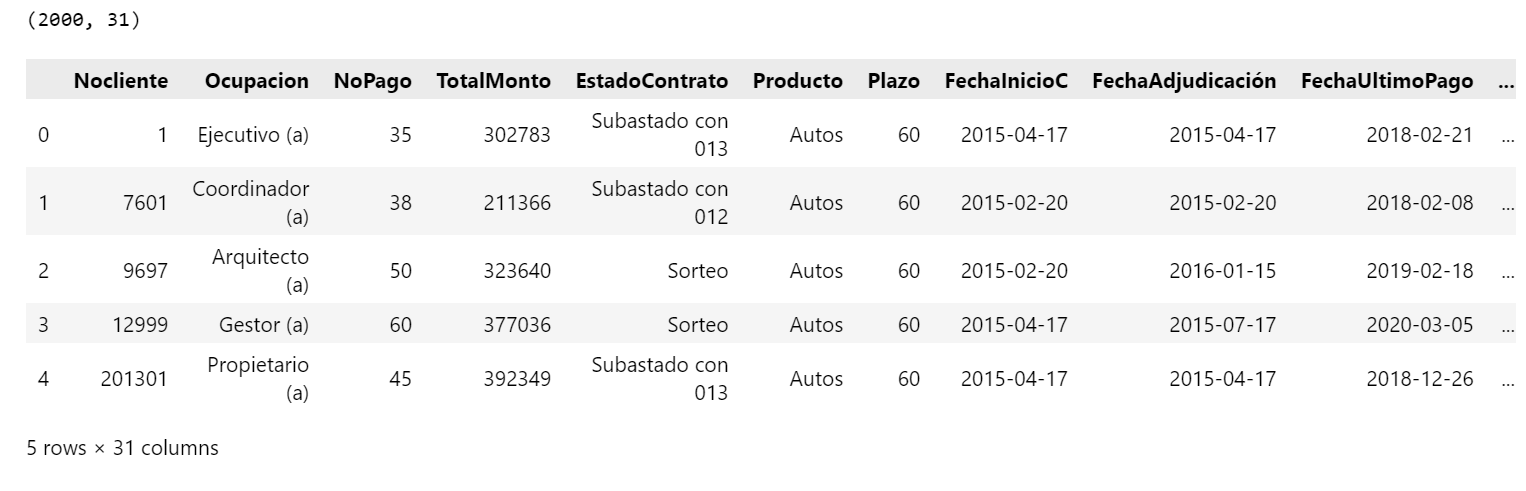
\includegraphics[width=14cm, height=8cm ]{Imagenes/DatasetLeido.PNG }
      \caption{Conjunto de datos o dataset leido}
      \label{fig:datasetl}
\end{figure}



Comenzaremos viendo las variables categóricas y numéricas usando la libreria Pandas y Python. Obtenemos la siguiente información como respuesta
\newpage
\begin{verbatim}
RangeIndex: 2000 entries, 0 to 1999 
Data columns (total 31 columns):
\end{verbatim}

\begin{table}[H]
    \centering
    
    \begin{tabular}{|c|c|c|c|c|}
        \hline
        \rowcolor{softblue} % Fila color azul suave
        \textbf{Num} & \textbf{Columna} & \textbf{Count} & \textbf{Non-Null} & \textbf{Dtype} \\
        \hline
        % \rowcolor{lightgray} % Fila color gris claro
        \hline
        0 &	Nocliente &		2000 &	non-null &	int64  \\
        \hline
        1 &	Ocupacion &		2000 &	non-null &	object \\
        \hline
        2 &  NoPago    &          2000 & non-null &  int64  \\
        \hline
        3 &  TotalMonto  &        2000 & non-null &  int64  \\
        \hline
        4 &  EstadoContrato &     2000 & non-null &  object \\
        \hline
        5 &   Producto  &         2000 & non-null &   object \\
        \hline
        6 &  Plazo     &          2000 & non-null &   int64  \\
        \hline
        7 &  FechaInicioC  &      2000 & non-null &   object \\
        \hline
        8 &  FechaAdjudicación &   2000 & non-null &   object \\
        \hline
        9 &   FechaUltimoPago &     2000 & non-null &   object \\
        \hline
        10 &  FechaProyectadaFin &  2000 & non-null &   object \\
        \hline
        11 &  MontoVencido &        2000 & non-null &   int64  \\
        \hline
        12 &  Mensualidad &         2000 & non-null &   int64  \\
        \hline
        \rowcolor{mediumgray}
        13 &  Ingresos &            1958 & non-null &   float64 \\
        \hline
        \rowcolor{mediumgray}
        14 &  Legal &               520 & non-null &    object \\
        \hline
        15 &  EdadActual &          2000 & non-null &   int64  \\
        \hline
        \rowcolor{mediumgray}
        16 &  FechaDEfiniquito &    0 & non-null &      float64 \\
        \hline
        17 &  AZULEstatus &         2000 & non-null &   object \\
        \hline
        \rowcolor{mediumgray}
        18 &  AdjudicaReal &        1457 & non-null &   object \\
        \hline
        19 &  PagosPuntuales &      2000 & non-null &   int64  \\
        \hline
        20 &  CostoAdmin &          2000 & non-null &   int64  \\
        \hline
        21 &  Genero &              2000 & non-null &   object \\
        \hline
        22 &  PersonaTipo &         2000 & non-null &   object \\
        \hline
        23 &  dtEstadoContrato &    2000 & non-null &   object \\
        \hline
        24 &  GrupoOrigenVenta &    2000 & non-null &   object \\
        \hline
        25 &  SemanasAdjud &        2000 & non-null &   float64 \\
        \hline
        26 &  Pagos9 &              2000 & non-null &   int64  \\
        \hline
        27 &  DomiciliaPago &      2000 & non-null &   int64  \\
        \hline
        28 &  Email &               2000 & non-null &   int64  \\
        \hline
        29 &  timetotV &            2000 & non-null &   int64  \\
        \hline
        30 &  Y &                   2000 & non-null &   int64 \\
        \hline  
    \end{tabular}
    \caption{Tabla con las variables numéricas y categóricas}
    \label{tab:vaxxx}
\end{table} \medskip

La tabla \ref{tab:vaxxx}  muestra que trabajaremos con un conjunto de datos de 2000 clientes y cada cliente con 30 columnas o variables. 
Además, nos indica la cantidad de información disponible en cada variable o columna. 
Si el tipo de dato (Dtype) es ''object'', la columna es categórica; de lo contrario, es una variable numérica.\medskip

Las variables numéricas son (int64 , float64):\medskip

NoPago, TotalMonto, MontoVencido, Mensualidad, Ingresos, EdadActual, CostoAdmin, SemanasAdjud,  Pagos9, Domicilia\_Pago, Email, timetotV \medskip

Y las variables categóricas (object):\medskip

Ocupacion, EstadoContrato, Producto, Legal, AZULEstatus,AdjudicaReal, Genero, PersonaTipo, dtEstadoContrato, GrupoOrigenVenta \medskip

Seguiremos los siguientes pasos sugeridos por Bronwnle J. \cite{Brown1} : \medskip
\begin{itemize}
    \item Eliminación de columnas con un único valor.
    \item Consideración de columnas con pocos valores únicos.
    \item Eliminación de columnas con baja variación.
    \item Identificación y eliminación de filas con datos duplicados.
    \item Eliminación de valores extremos (outliers) en caso de variables numéricas.
    \item Estandarización de errores tipográficos en variables categóricas.
\end{itemize}



\subsection{Eliminar columnas que contienen un solo valor} 

    La columna 'FechaDEfiniquito' no contiene información , ademas la columna 'Plazo' 
    solo tiene un valor y 'Nocliente' no es necesario, por lo que las eliminamos.
    

\subsection{ Considerar y/o eliminar columnas que tienen muy pocos valores}

En la tabla \ref{tab:vaxxx} vemos las variables que tienen menos información en un color gris mas oscuro. \medskip

Completamos y corregimos estas columnas usando las siguientes reglas del negocio: \medskip

\begin{itemize}
    \item Si el ingreso del cliente es menor o igual a 3,500 pesos, subimos a $ 4 * 3,500 $.
    \item La edad de cliente debe ser siempre mayor o igual a 18 años.
    \item La mensualidad debe ser siempre menor o igual ingreso.
    \item La variable o columna Legal debe tener uno de los valores Legal o Normal.
\end{itemize}

\subsection{ Identificar y eliminar filas duplicadas}

Dado que los clientes tienen un numero unico asignado, este proceso no se realiza. \medskip
\subsection{ Eliminación de valores extremos (outliers) en caso de variables numéricas}

En la siguiente tabla podemos ver los valores fuera de rango o outliers. \medskip
\newpage
\begin{figure}[H]
    \centering
       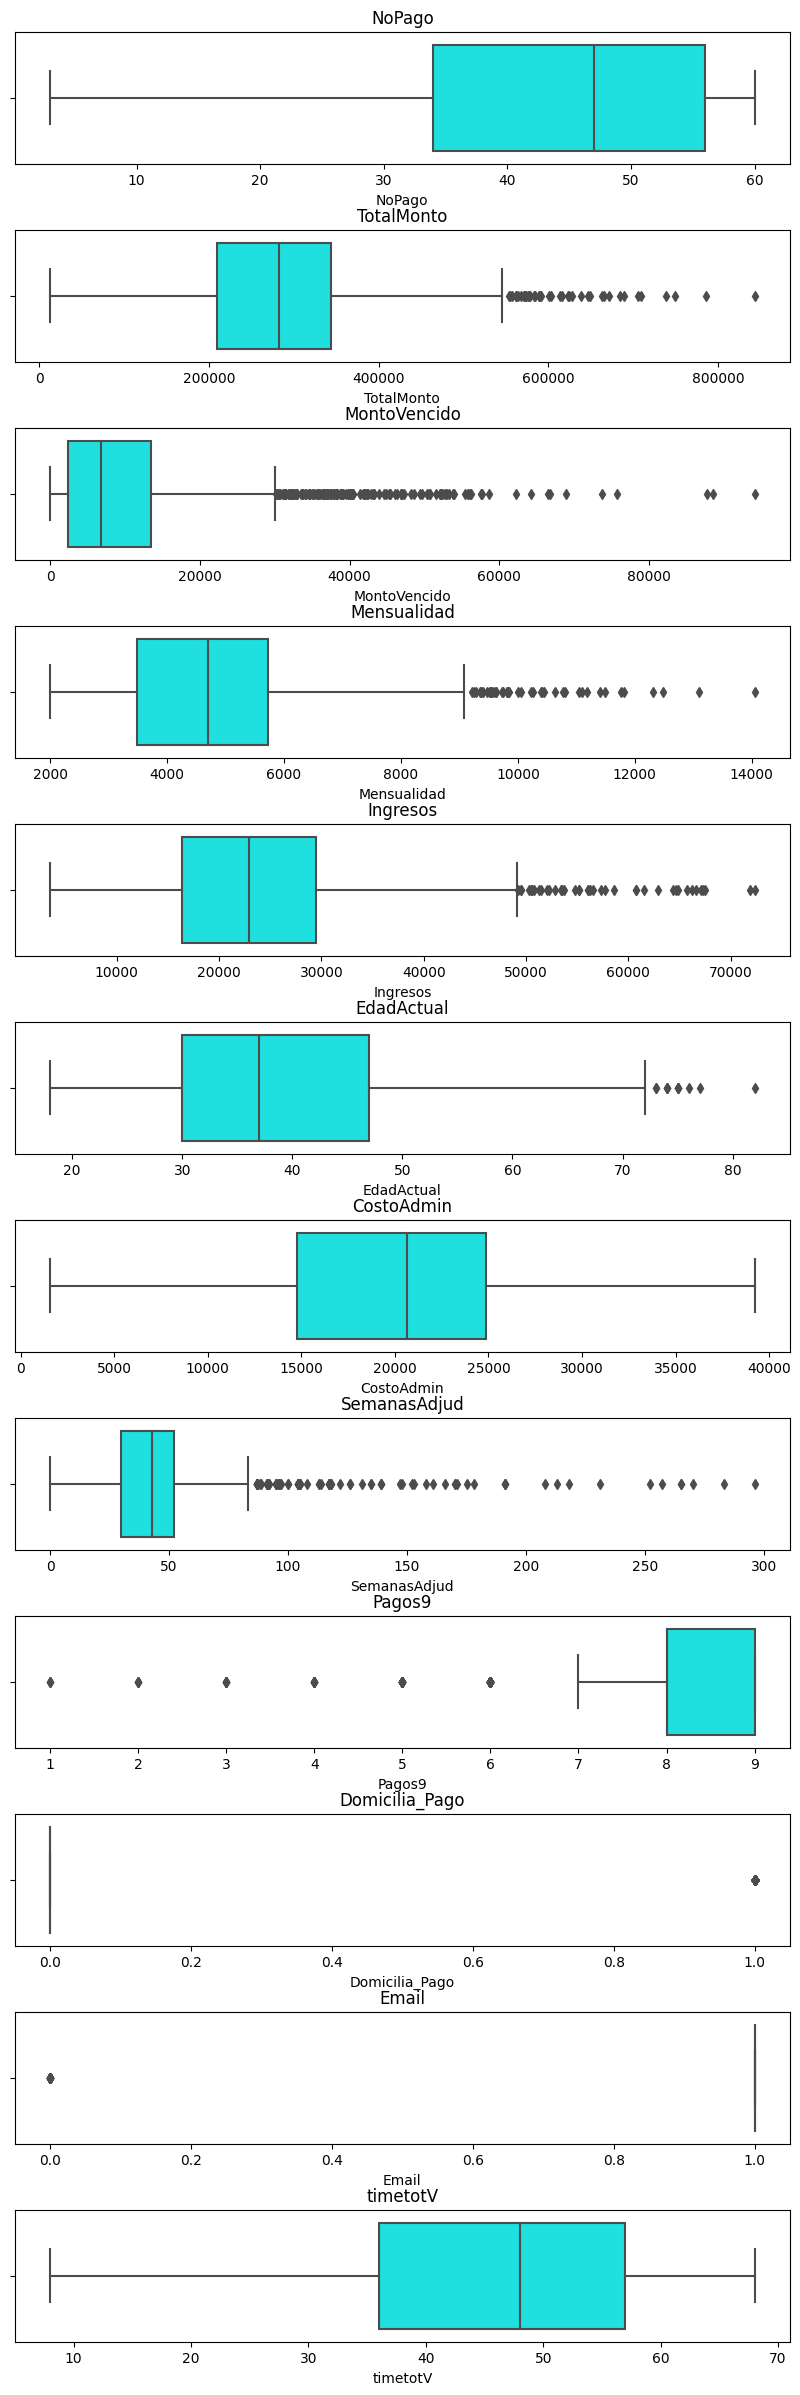
\includegraphics[width=16cm, height=21cm ]{Imagenes/GraficaCajaYBigoteNumericas.png}
      \caption{Valores fuera de rango o outliers}
      \label{fig:Outliers}
\end{figure}

De la figura \ref{fig:Outliers} consideramos que los valores numéricos fuera de rango son aceptables.

Las variables categóricas se ponen en minúsculas y en la figura \ref{fig:NivelesCate} , podemos observar 
los niveles o valores distintos que toma una variables categórica. \medskip
\begin{figure}[H]
    \centering
       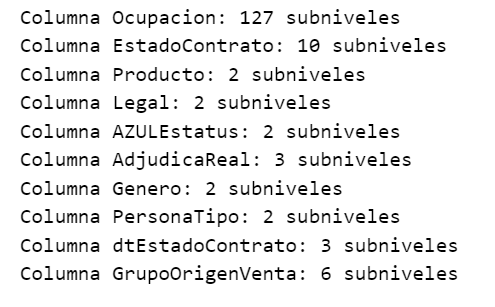
\includegraphics[width=12cm, height=5cm ]{Imagenes/SubNivelesCategoricas.PNG}
      \caption{Niveles o valores que toma una variables categórica}
      \label{fig:NivelesCate}
\end{figure}

Se detecta cualquier anomalía mediante las graficas de barras de cada una de ellas.\medskip

\begin{figure}[H]
    \centering
       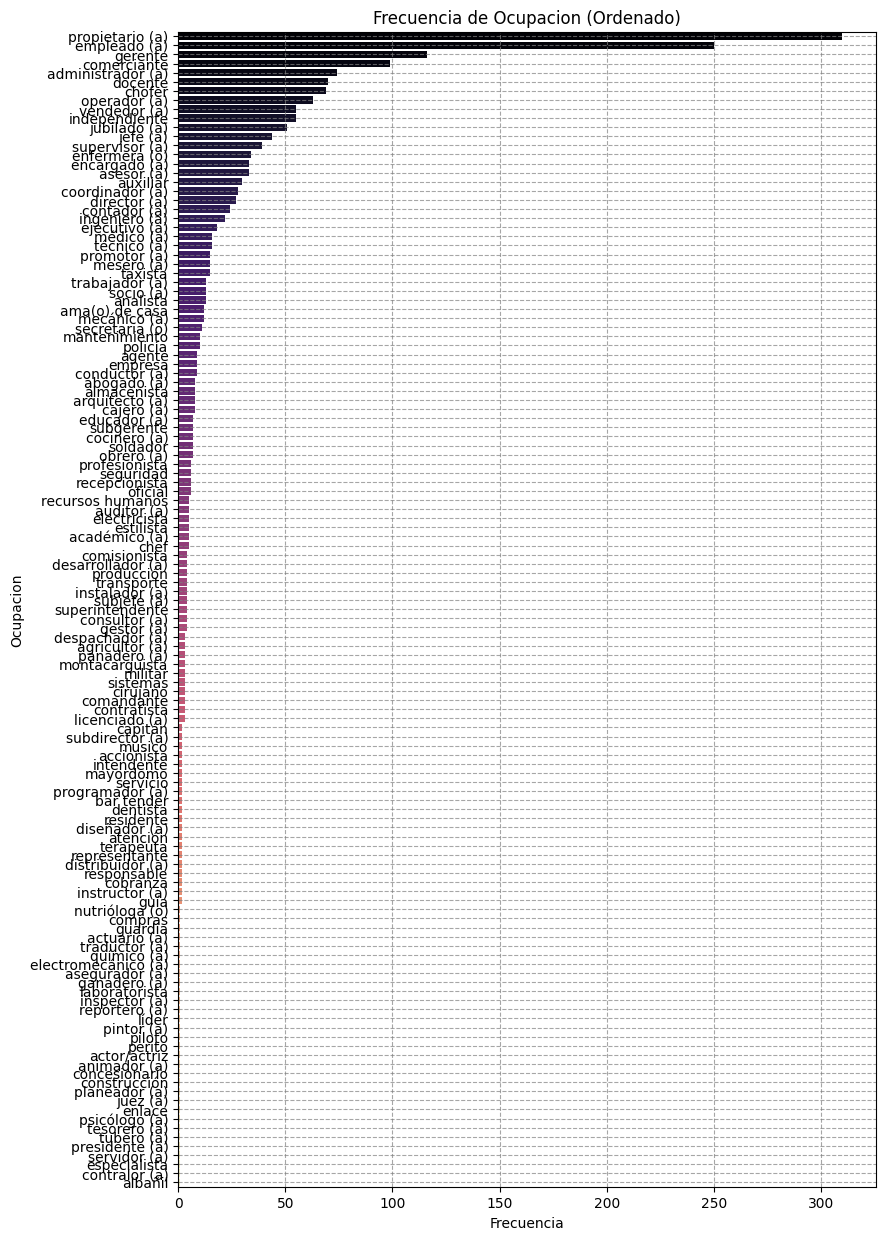
\includegraphics[width=14cm, height=21cm ]{Imagenes/Ocupacion.png}
      \caption{Grafica de ocupación del cliente vs frecuencia}
      \label{fig:Ocupacion}
\end{figure}

\begin{figure}[H]
    \centering
       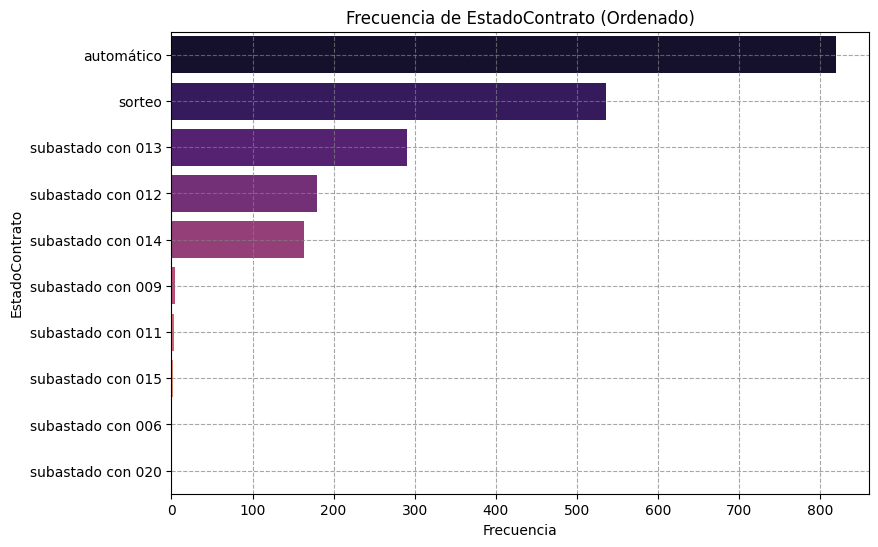
\includegraphics[width=14cm, height=10cm ]{Imagenes/EstadoContrato.png}
      \caption{Grafica de estado de contrato  vs frecuencia}
      \label{fig:Edocontra}
\end{figure}
\begin{figure}[H]
    \centering
       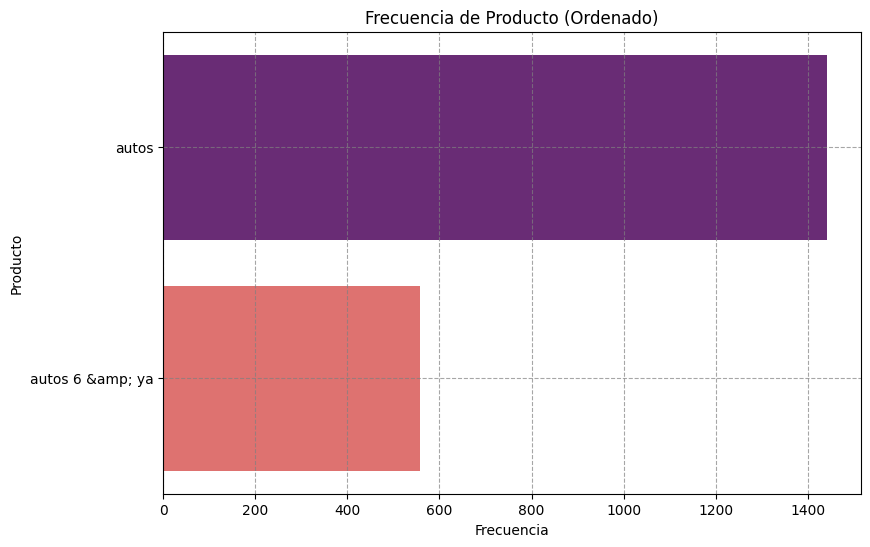
\includegraphics[width=14cm, height=10cm ]{Imagenes/Producto.png}
      \caption{Grafica de producto  vs frecuencia}
      \label{fig:ProductoF}
\end{figure}

\section{Medidas Estadísticas}

Determinamos la estadística básica del dataset, calculando para las variables numéricas

\begin{itemize}
    \item Promedio (mean).
    \item Desviación estandard (std).
    \item Valor mínimo.
    \item Valor máximo.
    \item Cuartiles (25\%, 50\% y 75\%).
\end{itemize} \medskip


\begin{figure}[H]
    \centering
       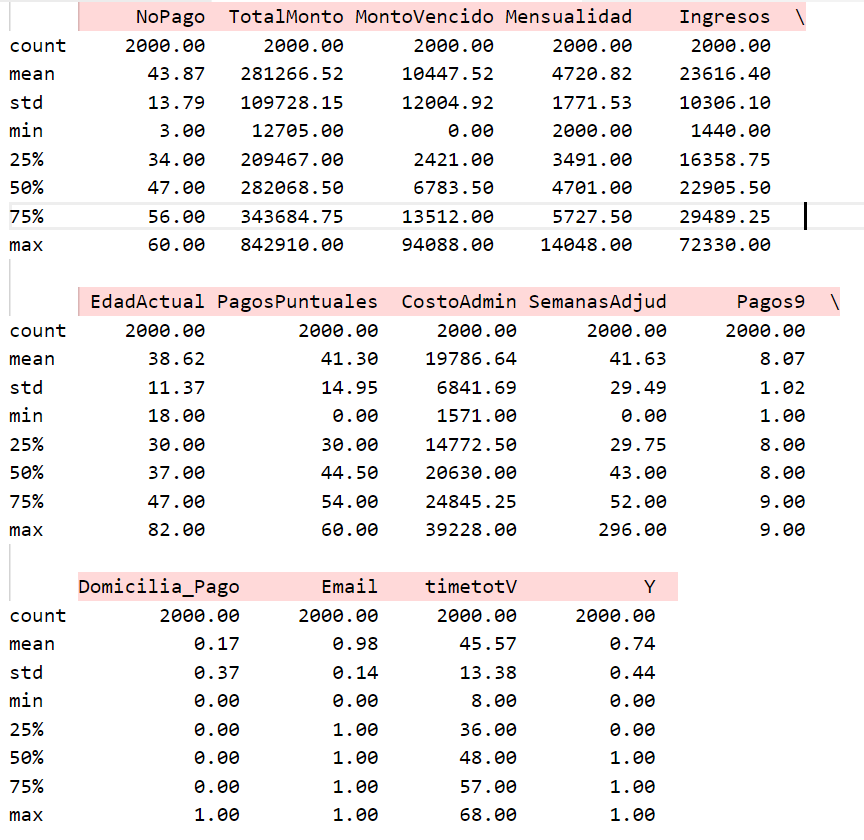
\includegraphics[width=14cm, height=16cm ]{Imagenes/EstadisticaBasica.PNG}
      \caption{Estadística básica para variables numéricas}
      \label{fig:EstBasica}
\end{figure}

\section{Correlación entre variables}

\begin{figure}[H]
    \centering
       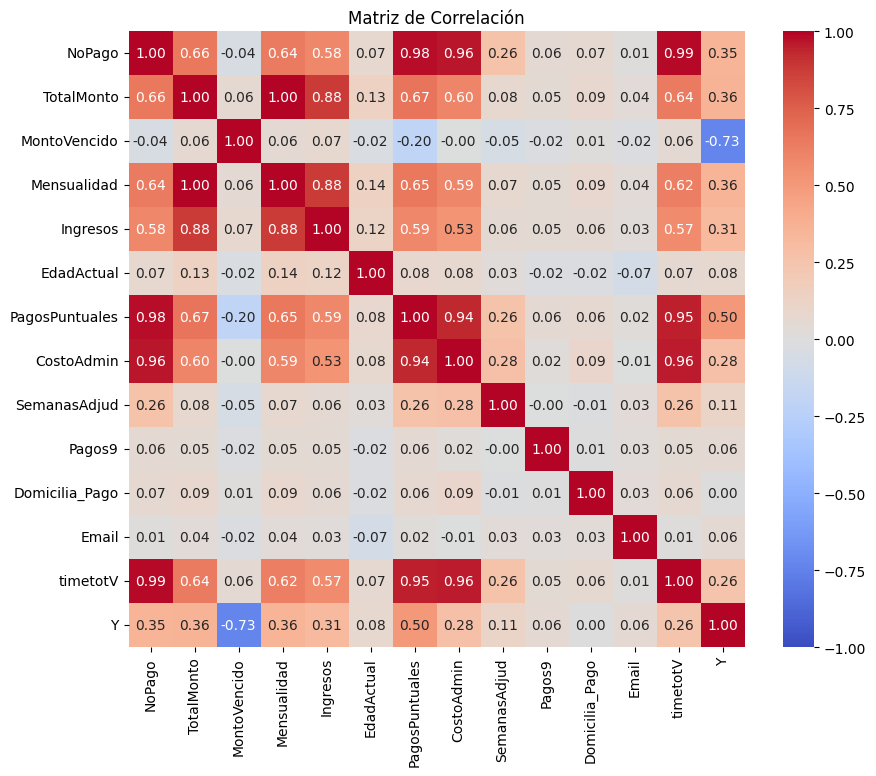
\includegraphics[width=14cm, height=14cm ]{Imagenes/Correlaciones.png}
      \caption{Correlaciones entre variables numéricas}
      \label{fig:Corres}
\end{figure}

Finalmente se guarda el dataset limpio en el archivo : ``Clientes\_Dos\_Mil\_Limpio.csv''.


\section{Transformación del dataset}
Para que un algoritmo de machine learning funcione bien, es crucial que los datos de entrada estén 
en el formato adecuado. En la mayoría de los casos, estos algoritmos requieren datos en formato 
numérico para realizar sus cálculos.\medskip

El proceso de adaptar o transformar los datos para que sean compatibles con el algoritmo se llama 
preprocesamiento y transformación de datos.

\subsection{Transformación StandardScaler}
Es el proceso mediante el cual un conjunto de datos se transforma para que siga una distribución normal
con media 0 y desviación estándar 1. \medskip

Matemáticamente : $ x_i' = \displaystyle {\frac{x_i - \mu}{\sigma}} $ \medskip

Con scikit-learn : \medskip

\begin{tcolorbox}[colback=gray!30, coltext=black, colframe=black, boxrule=0.5mm, width=\textwidth]
    \begin{verbatim}
        from sklearn.preprocessing import StandardScaler
        X_transformado = StandardScaler().fit_transform(X)
    \end{verbatim}
\end{tcolorbox}

De forma grafica podemos ver en la siguiente figura \ref{fig:crudoAstandar} , en que consiste la transformación

\begin{figure}[h!]
    \centering
    \begin{minipage}{0.45\textwidth}
        \centering
        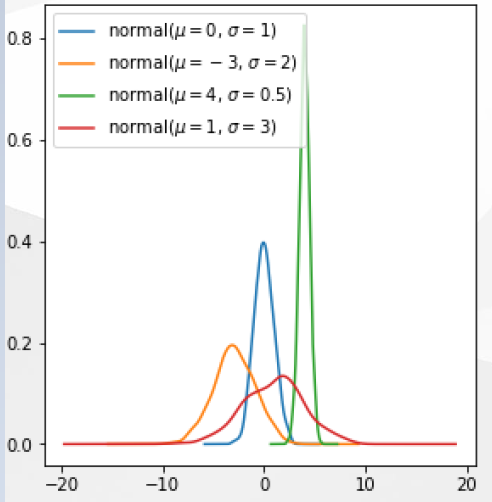
\includegraphics[width=\linewidth]{Imagenes/StandarCrudo.PNG}
        \caption{Datos en crudo}
        \label{fig:DatosCru}
    \end{minipage}
    \hspace{0.05\textwidth}
    \begin{minipage}{0.45\textwidth}
        \centering
        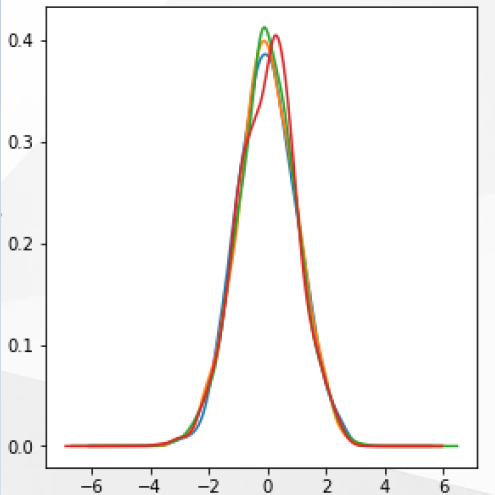
\includegraphics[width=\linewidth]{Imagenes/StandarNormalizado.PNG}
        \caption{StandardScaler}
        \label{fig:figura2}
    \end{minipage}
    \caption{Transformación de datos en crudo a StandardScaler}
    \label{fig:crudoAstandar}
\end{figure}

\subsection{Transformación OrdinalEnconder}

OrdinalEncoder asigna un valor numérico ordinal a cada categoría. De forma predeterminada, 
estos valores se asignan siguiendo el orden alfabético de las categorías. \medskip

Con scikit-learn : \medskip

\begin{tcolorbox}[colback=gray!30, coltext=black, colframe=black, boxrule=0.5mm, width=\textwidth]
    \begin{verbatim}
        from sklearn.preprocessing import OrdinalEncoder
        datos_transformados = encoder.fit_transform(datos)
    \end{verbatim}
\end{tcolorbox}

De forma grafica podemos ver en la siguiente figura \ref{fig:Orencoder} , la transformación de una
variable categórica a OrdinalEnconder. \medskip

\begin{figure}[H]
    \centering
       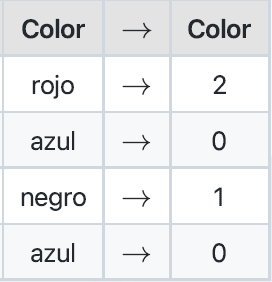
\includegraphics[width=4cm, height=5cm ]{Imagenes/Encoder.PNG}
      \caption{Transformación de una variable categórica a OrdinalEncoder}
      \label{fig:Orencoder}
\end{figure}

\section{Partición del dataset}

    \begin{figure} [H]
        \centering
        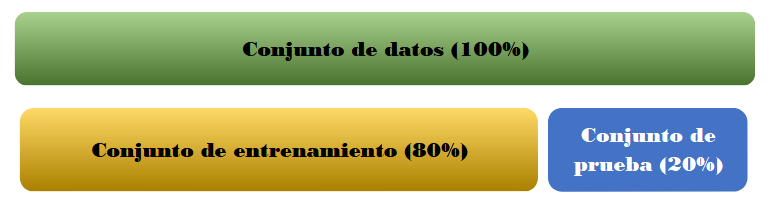
\includegraphics[width=12cm, height=4cm ]{Imagenes/ParticionDEdatos.PNG }
        \caption{Partición del dataset}
        \label{fig:parti}
    \end{figure}

    

\subsection{Partición del dataset}




% Obligatorio
\chapter{Resultados}\label{cap5:resultados}

\textcolor{blue}{[Aqui viene los Resultados.....solo copiar de word.]}
\bigskip
% Obligatorio
\chapter{Contribuciones, conclusiones y trabajos 
futuros}\label{cap6:conclusiones}


% Aqui vienen las Referencias formato Apa7
%\bibliographystyle{apalike}
%\bibliographystyle{Referencias/MisReferencias.bib}
%

\begin{thebibliography}{99}
  \bibitem{Bagnato} J.I. Bagnato. Aprende Machine Learning (Teoría + Práctica Python) . Lean Pub. 2020.
  \bibitem{Brownlee} J. Brownlee. Master Machine Learning Algorithms. eBook: Machine Learning Mastery. 2017.
  \bibitem{Raschka} Sebastian. Raschka, Python Machine Learning , México , Macrombo S.A., 2020.
  \bibitem{Vladi} Vladimirovna, O., y Gutierrez Gonzalez, E. ,Probabilidad y Estadística: Aplicaciones a la Ingeniería y Ciencias. Cdmx: Grupo Editorial Patria,2016.
  \bibitem{Gilb} Gilbert, S. , Álgebra Lineal en ciencia de datos. Wellesley-Cambridge Press, US, 2022.
  \bibitem{Kle} Klein, B. ,Data Analysis Numpy Matplotlib and Pandas, Python-course,EU, 2021.
  \bibitem{Gilbert} Gilbert, S. ,Linear Algebra for Everyone ,Wellesley-Cambrige Press MIT,US, 2020.
  \bibitem{Arang} Arangala C. ,Linear Algebra with Machine Lerning and data ,CRC Press,US, 2023.
  \bibitem{Simon} Simon R. Girolami M. , A First Course in Machine Learning ,CRC Press,US, 2017.
  \bibitem{Brown1} Bronwnle J. , Data Preparation for Machine Learning - Data Cleaning, Feature Selection, and Data Transforms in Python,eBook: Machine Learning Mastery , 2020
  \bibitem{Brown7} Bronwnle J. , Machine Learning Algorithms From Scratch With Python ,eBook: Machine Learning Mastery , 2020
  \bibitem{Cuevas} Cuevas E. Avalos O. Diaz P. , Introducción al Machine Learning con MatLab, Macrombo, México, 2022
  \bibitem{roh1} Rolando Ortiz Herbas , \url{https://github.com/RolandoOrtizHerbas/Proyecto-I-y-II-MatUNADM/blob/Rama01/Programas_Scripts_Jupiter/Limpieza_de_datos.ipynb} , Jupiter Python, México, 2024
\end{thebibliography}
\end{document}
